\section{\index{Stark!Stark Effect}{Stark Effect}}\label{stark}
For our Spin Hamiltonian given by 
\begin{equation}
    \begin{align}
        H &= H_{\ce{ZFS}} + H_{\ce{Zeeman}} + H_{\ce{Hyperfine}} + H_{\ce{Zeeman(n)}}+ H_{\ce{Quadrupole}}\\ 
        H &= \hat{\vec{S}}\cdot{\vec{D}}\cdot{\vec{S}} + g\mu_b \hat{\vec{S}}\cdot \vec{B}  + \hat{\vec{S}}\cdot A \cdot \hat{\vec{I}}  -  \mu_n g_n \hat{\vec{I}}\cdot\vec{B} + \hat{\vec{I}} \cdot Q \cdot \hat{\vec{I}}.
    \end{align}
    % \label{eq:}
\end{equation}
In the most general sense, an applied electrical field could change any of the parameters. We will not consider the effect of an applied electrical field on the nuclear Zeeman term as the nuclear is \index{paramagnetically shielded}{paramagnetically shielded} \cite{mims}. 
Thus, in a general sense we may add the contributions of an applied electrical field $\vec{E}$ as $H + H_{\ce{Stark}}$ where 
\begin{equation}
    H_{\ce{Stark}} = \vec{E}\cdot\left(\hat{\vec{S}}\cdot R \cdot \hat{\vec{S}} + T \mu_B \hat{\vec{S}}\cdot \vec{B} + \hat{\vec{S}}\cdot F \cdot \hat{\vec{I}} + \hat{\vec{I}} \cdot q \cdot \hat{\vec{I}} \right). 
    \label{eq:}
\end{equation}%

Here $R, T, F, q$ are matrices for each component of the electric field given by 
\begin{equation}
    R_{ijk} = \frac{\partial D_{jk}}{\partial E_i}, \quad 
    T_{ijk} = \frac{\partial g_{jk}}{\partial E_i}, \quad 
    F_{ijk} = \frac{\partial A_{jk}}{\partial E_i}, \quad 
    q_{ijk} = \frac{\partial Q_{jk}}{\partial E_i}.
    \label{eq:}
\end{equation}

We may immediately simplify $T$ as for this work we assume isotropic and constant $g$, for which $T$ is zero.  

Further, as discussed in section \ref{nuclear} we will not include the contributions of the nuclear Hamiltonians. 

This allows us to then consider only the energy change due to the shift in the $D$ parameter, that is $R$, which is a square matrix for each component of the applied $\vec{E}$. 
Exactly as we did for ZFS in section \ref{zfs}, we may reduce each of these symmetric matrices to a traceless form. 
% Here we define $D$ and $E$ in exactly the same way as \ref{}\td{link D E def}. 

% Additionally, each matrix $R$ must be symmetric, that is $R^T = R$ since the matrix $D$ in the ZFS Hamiltonian is always symmetric. 

Consider the expansion of $\hat{\vec{S}}\cdot R \cdot \hat{\vec{S}}$ which we calculate explicitly 
\begin{equation}
    \begin{align}
        \hat{\vec{S}}\cdot R \cdot \hat{\vec{S}} &= 
    \begin{pmatrix}
        \hat{S}_x & \hat{S}_y & \hat{S}_z
    \end{pmatrix}
    \cdot 
    \begin{pmatrix}
        R_{xx} & R_{xy} & R_{xz} \\
        R_{xy} & R_{yy} & R_{yz} \\
        R_{xz} & R_{yz} & R_{zz} \\
    \end{pmatrix}
    \cdot 
    \begin{pmatrix}
        \hat{S}_x \\ \hat{S}_y \\ \hat{S}_z
    \end{pmatrix}\\ 
         &= R_{xx} \hat{S}_x^2  + R_{yy} \hat{S}_y^2 + R_{zz} \hat{S}_z^2 \\
         &+   R_{xy}(\hat{S}_{x}\hat{S}_y + \hat{S}_y \hat{S}_x) 
        +   R_{xz}(\hat{S}_{x}\hat{S}_z + \hat{S}_z \hat{S}_x) 
        +   R_{yz}(\hat{S}_{y}\hat{S}_z + \hat{S}_z \hat{S}_y).
    \end{align}
    \label{eq:}
\end{equation}

We set the constant trace equal to zero and rewrite 
\begin{equation}
 R_{xx} \hat{S}_x^2  + R_{yy} \hat{S}_y^2 + R_{zz} \hat{S}_z^2   = R_D \left(\hat{S}_z^2 - \frac{1}{3}S(S+1)\right) + R_E\left(\hat{S}_x^2 - \hat{S}_y^2\right).
    \label{eq:}
\end{equation}
Where \index{Stark!$R_D$}{$R_D$} and \index{Stark!$R_E$}{$R_E$} are defined in terms of $R$ the same way $D$ and $E$ are in terms of $D$, see \eqref{fs_D}, \eqref{fs_E}. 

Then, we may write $H_{\ce{Stark}}$ in this basis as 
\begin{equation}
    \begin{align}
        H_{\ce{Stark}} &=\vec{E} \cdot \Biggl(  R_D \left(\hat{S}_z^2 - \frac{1}{3}S(S+1)\right) + R_E\left(\hat{S}_x^2 - \hat{S}_y^2\right) \\ &+ 
   R_{xy}(\hat{S}_{x}\hat{S}_y + \hat{S}_y \hat{S}_x) 
        +   R_{xz}(\hat{S}_{x}\hat{S}_z + \hat{S}_z \hat{S}_x) 
        +   R_{yz}(\hat{S}_{y}\hat{S}_z + \hat{S}_z \hat{S}_y) \Biggr).
    \end{align}
    \label{eq:}
\end{equation}

The final step is to reduce the number of coefficients by exploiting the symmetry of the system. We will study systems with the \index{point group symmetry}{point group symmetry} of $C_{3v}$ \cite{Davidsson2018} which reduces the Hamiltonian again to \cite{mims}
\begin{equation}
    \begin{align}
        H_{\ce{Stark}} &= R_{113}\left(E_x (\hat{S}_x\hat{S}_y + \hat{S}_z\hat{S}_x) + E_y(\hat{S}_y\hat{S}_z + \hat{S}_z\hat{S}_y) \right) \\ 
                       &- R_{2E} \left(E_x(\hat{S}_x\hat{S}_y + \hat{S}_y\hat{S}_x) + E_y(\hat{S}_x^2 - \hat{S}_y^2   )\right) \\ 
                       &+ R_{3D}E_z\left(\hat{S}_z^2 - \frac{1}{3} S(S+1)\right)
    \end{align}
    \label{eq:}
\end{equation}


The coefficient $R_{113}$ represents a mixing of the $m_S = 0$ and $m_S = \pm 1$ states which have an energy splitting of $\mathcal{O}(10^9)$ Hz. The Stark energies are $\sim \mathcal{O} (10^3)$ Hz and of at least second order, thus may be ignored \cite{VanOort1990}.  

Thus finally, we write our \index{Stark!Stark Hamiltonian}{Stark Hamiltonian} as 

\begin{equation}
    \begin{align}
        H_{\ce{Stark}} &=
                        d_\parallel E_z\left(\hat{S}_z^2 - \frac{1}{3} S(S+1)\right)
        - d_\perp  E_y(\hat{S}_x^2 - \hat{S}_y^2   ) + d_\perp E_x(\hat{S}_x\hat{S}_y + \hat{S}_y\hat{S}_x)  
    \end{align}
    \label{eq:stark_hamiltonian}
\end{equation}

where we have labelled the axial contribution as \index{Stark!$d_\parallel$}{$d_\parallel$} and the off-axis contribution as \index{Stark!$d_\perp$}{$d_\perp$} to match the convention of existing literature. 

By direct comparison to \eqref{eq:ZFS_hamiltonian} it is easy to see the first two terms of $\eqref{eq:stark_hamiltonian}$ will contribute to the effective ZFS.  

In general longitudinal fields along the defect’s symmetry axis result in equal shifts of all levels, whereas transverse fields split the orbitals into two branches whose energy difference grows with increasing field \cite{Acosta2012, Bassett2011}. This allows the parameters $d_\perp$ and $d_\parallel$ to be measured experimentally. 

\begin{figure}[H]
    \begin{center}
        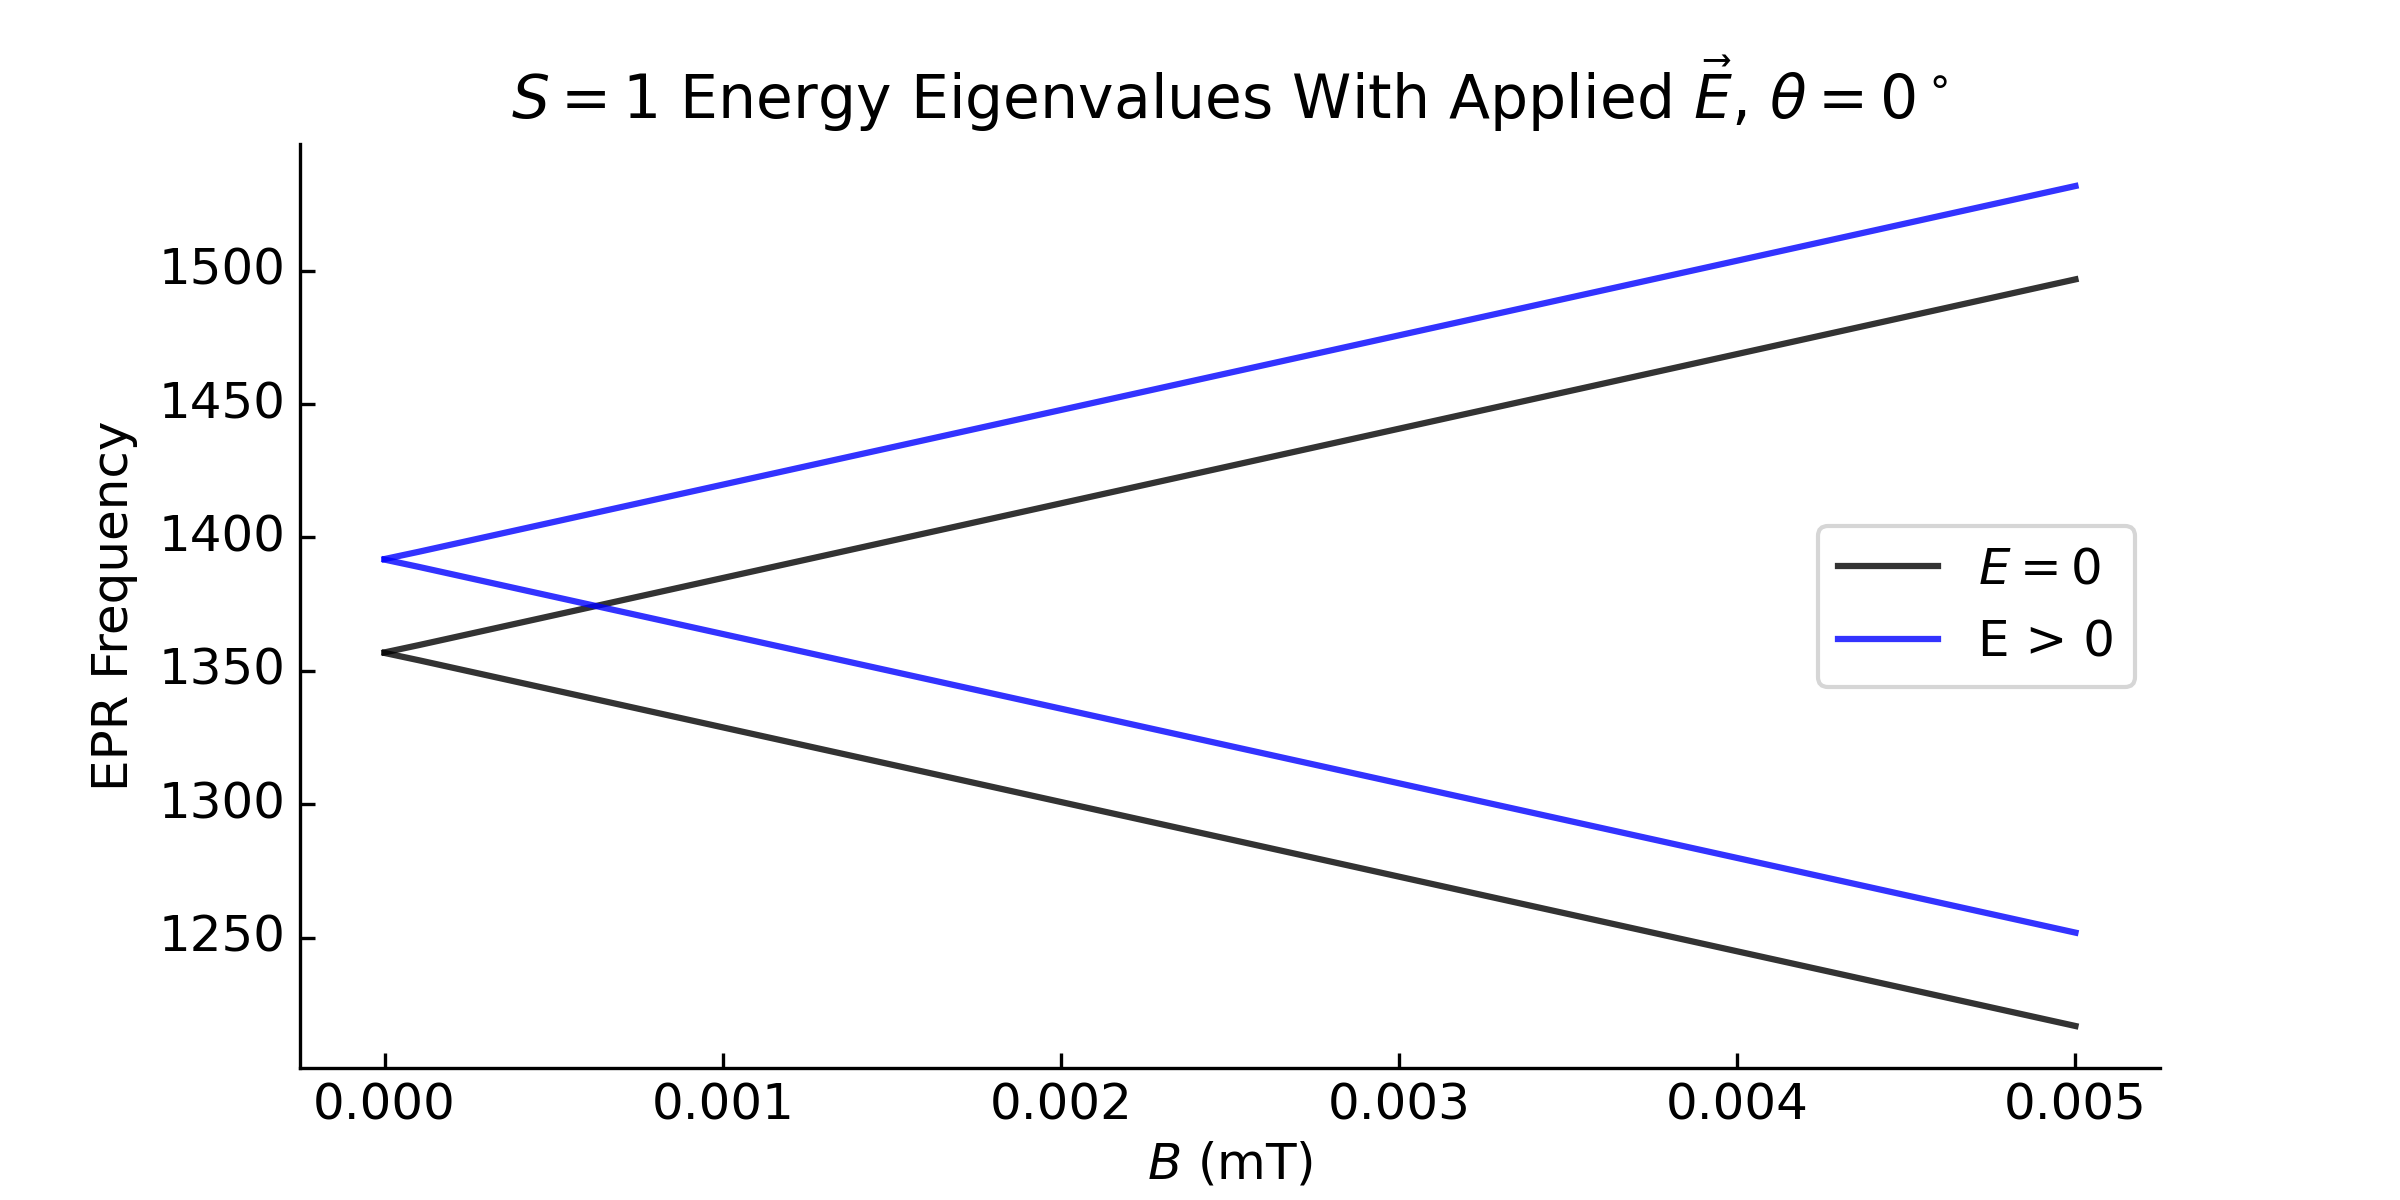
\includegraphics[width=0.95\textwidth]{figures/EFieldParallel.png}
        % 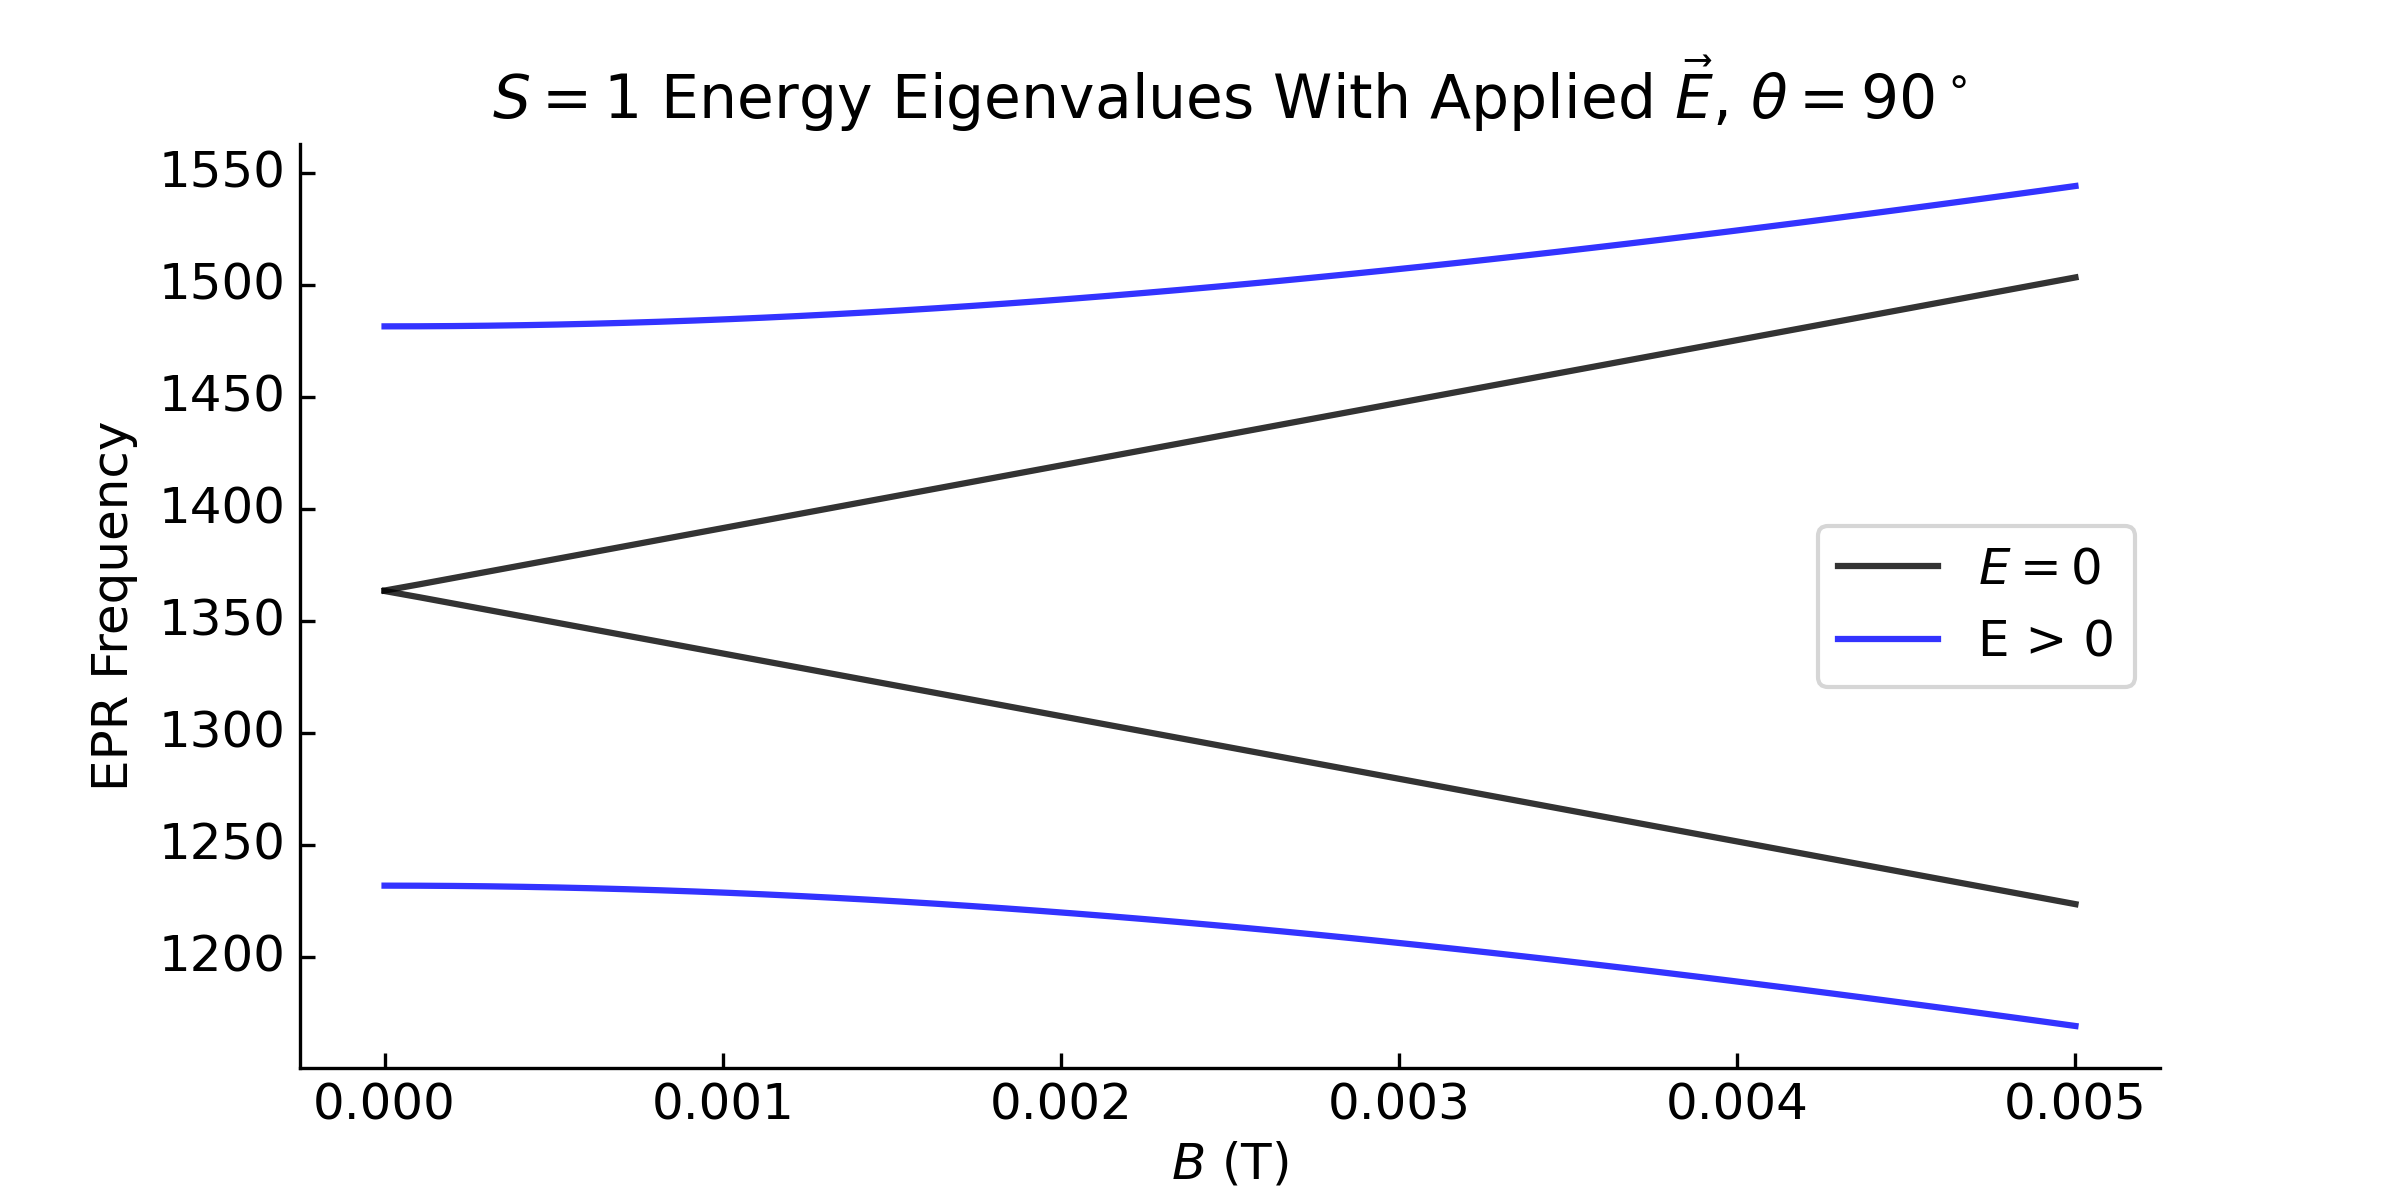
\includegraphics[width=0.95\textwidth]{figures/EFieldPerp.png}
        % \missingfigure{ODMR/Energy plot showing effect of parallel/perp E field}
    \end{center}
    \caption{Eigenvalue plot showing... \td{better caption}}\label{fig:}
\end{figure}
\begin{figure}[H]
    \begin{center}
        % 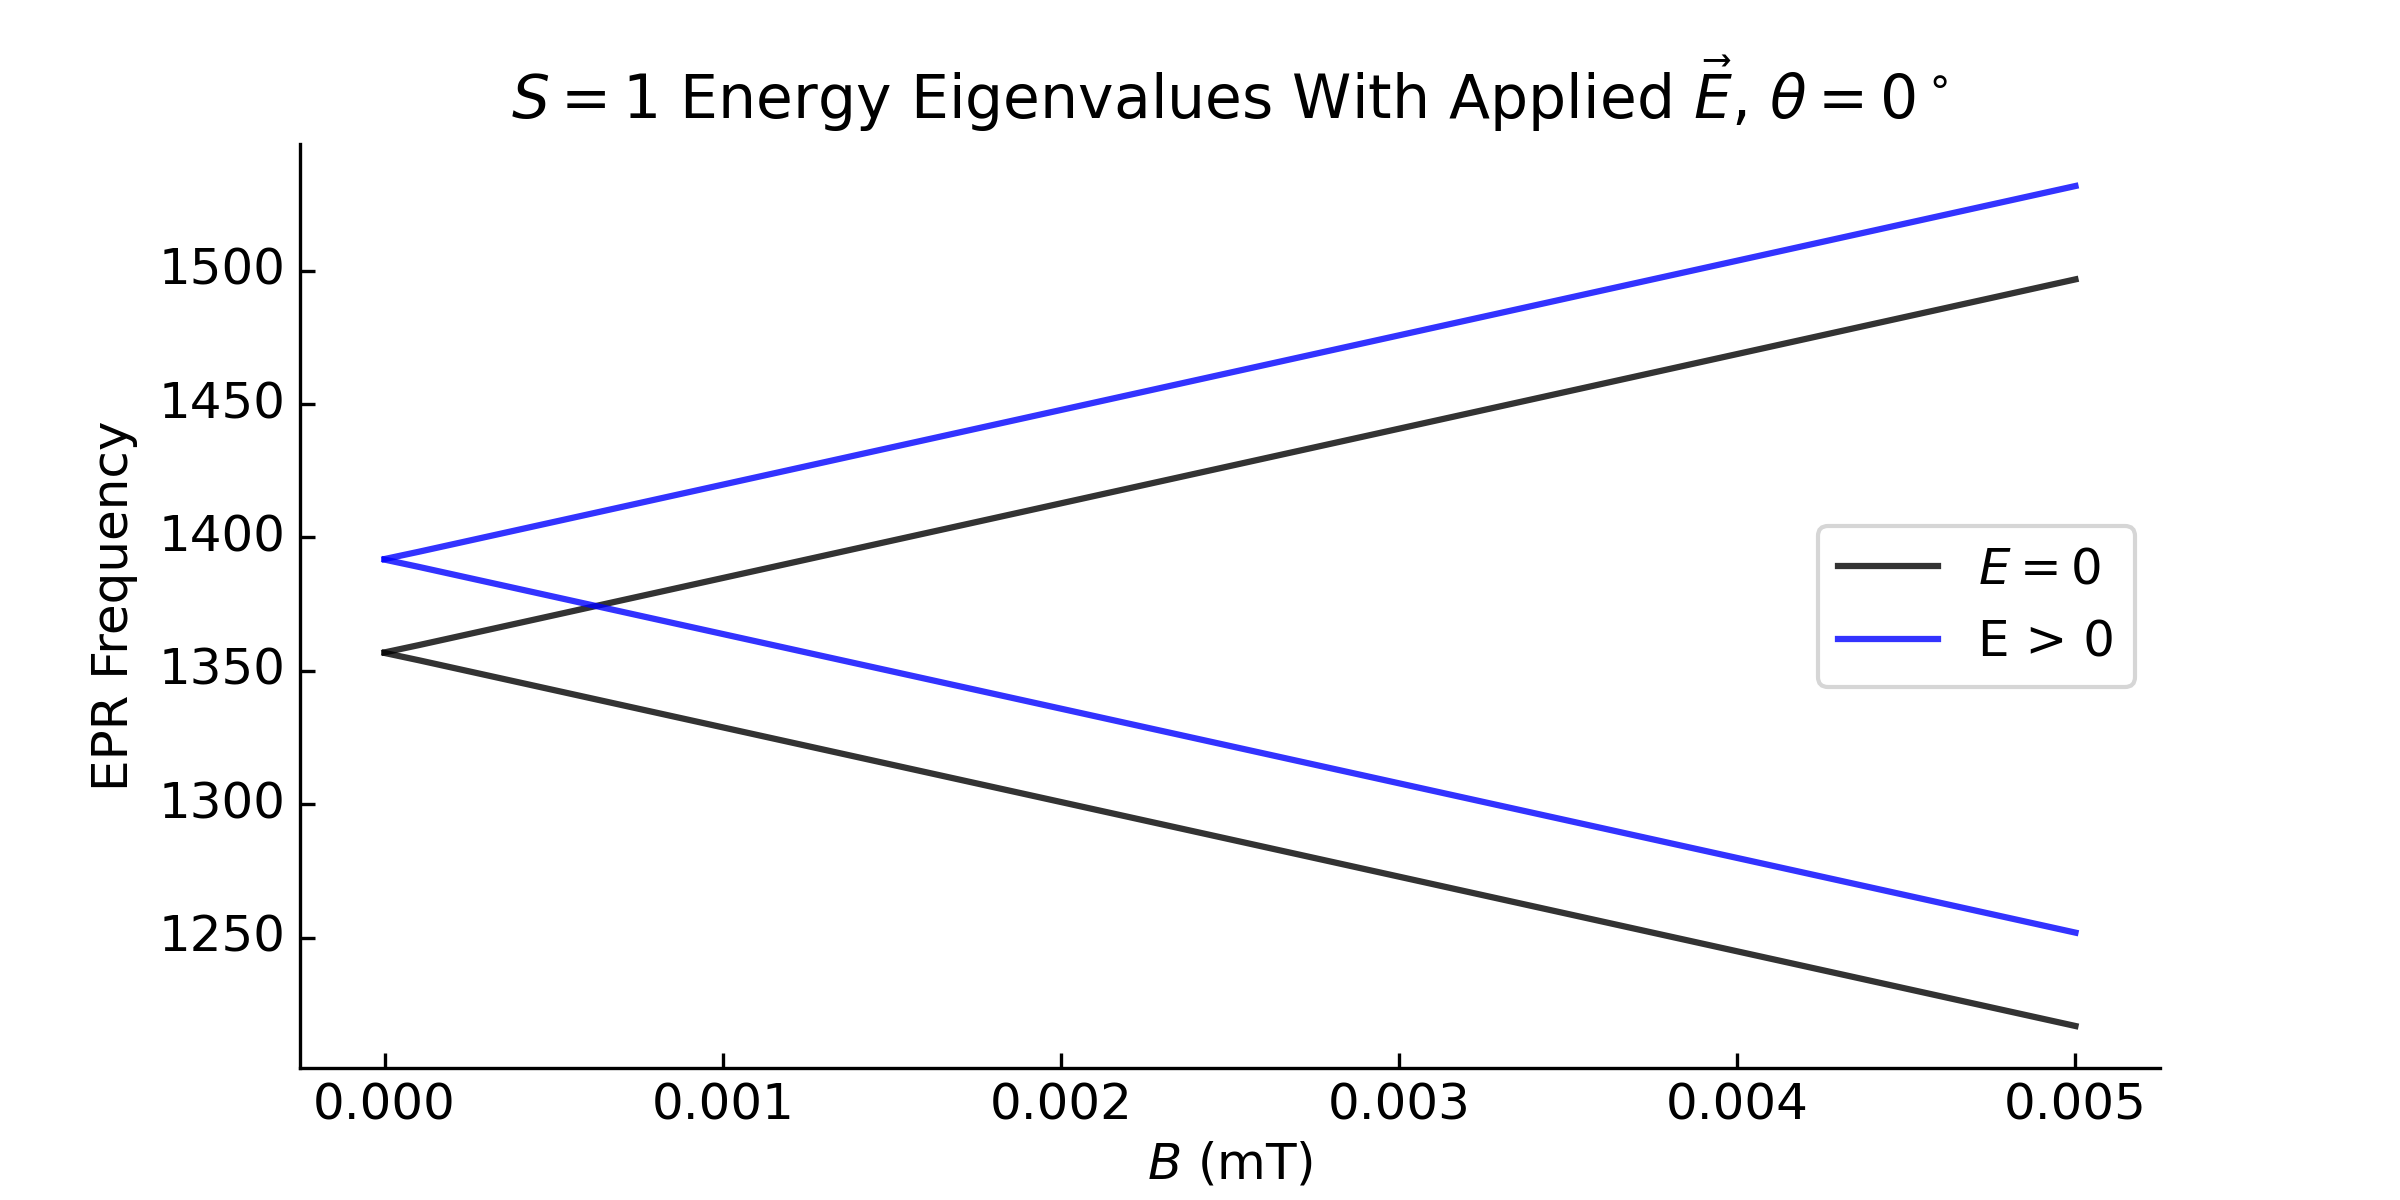
\includegraphics[width=0.95\textwidth]{figures/EFieldParallel.png}
        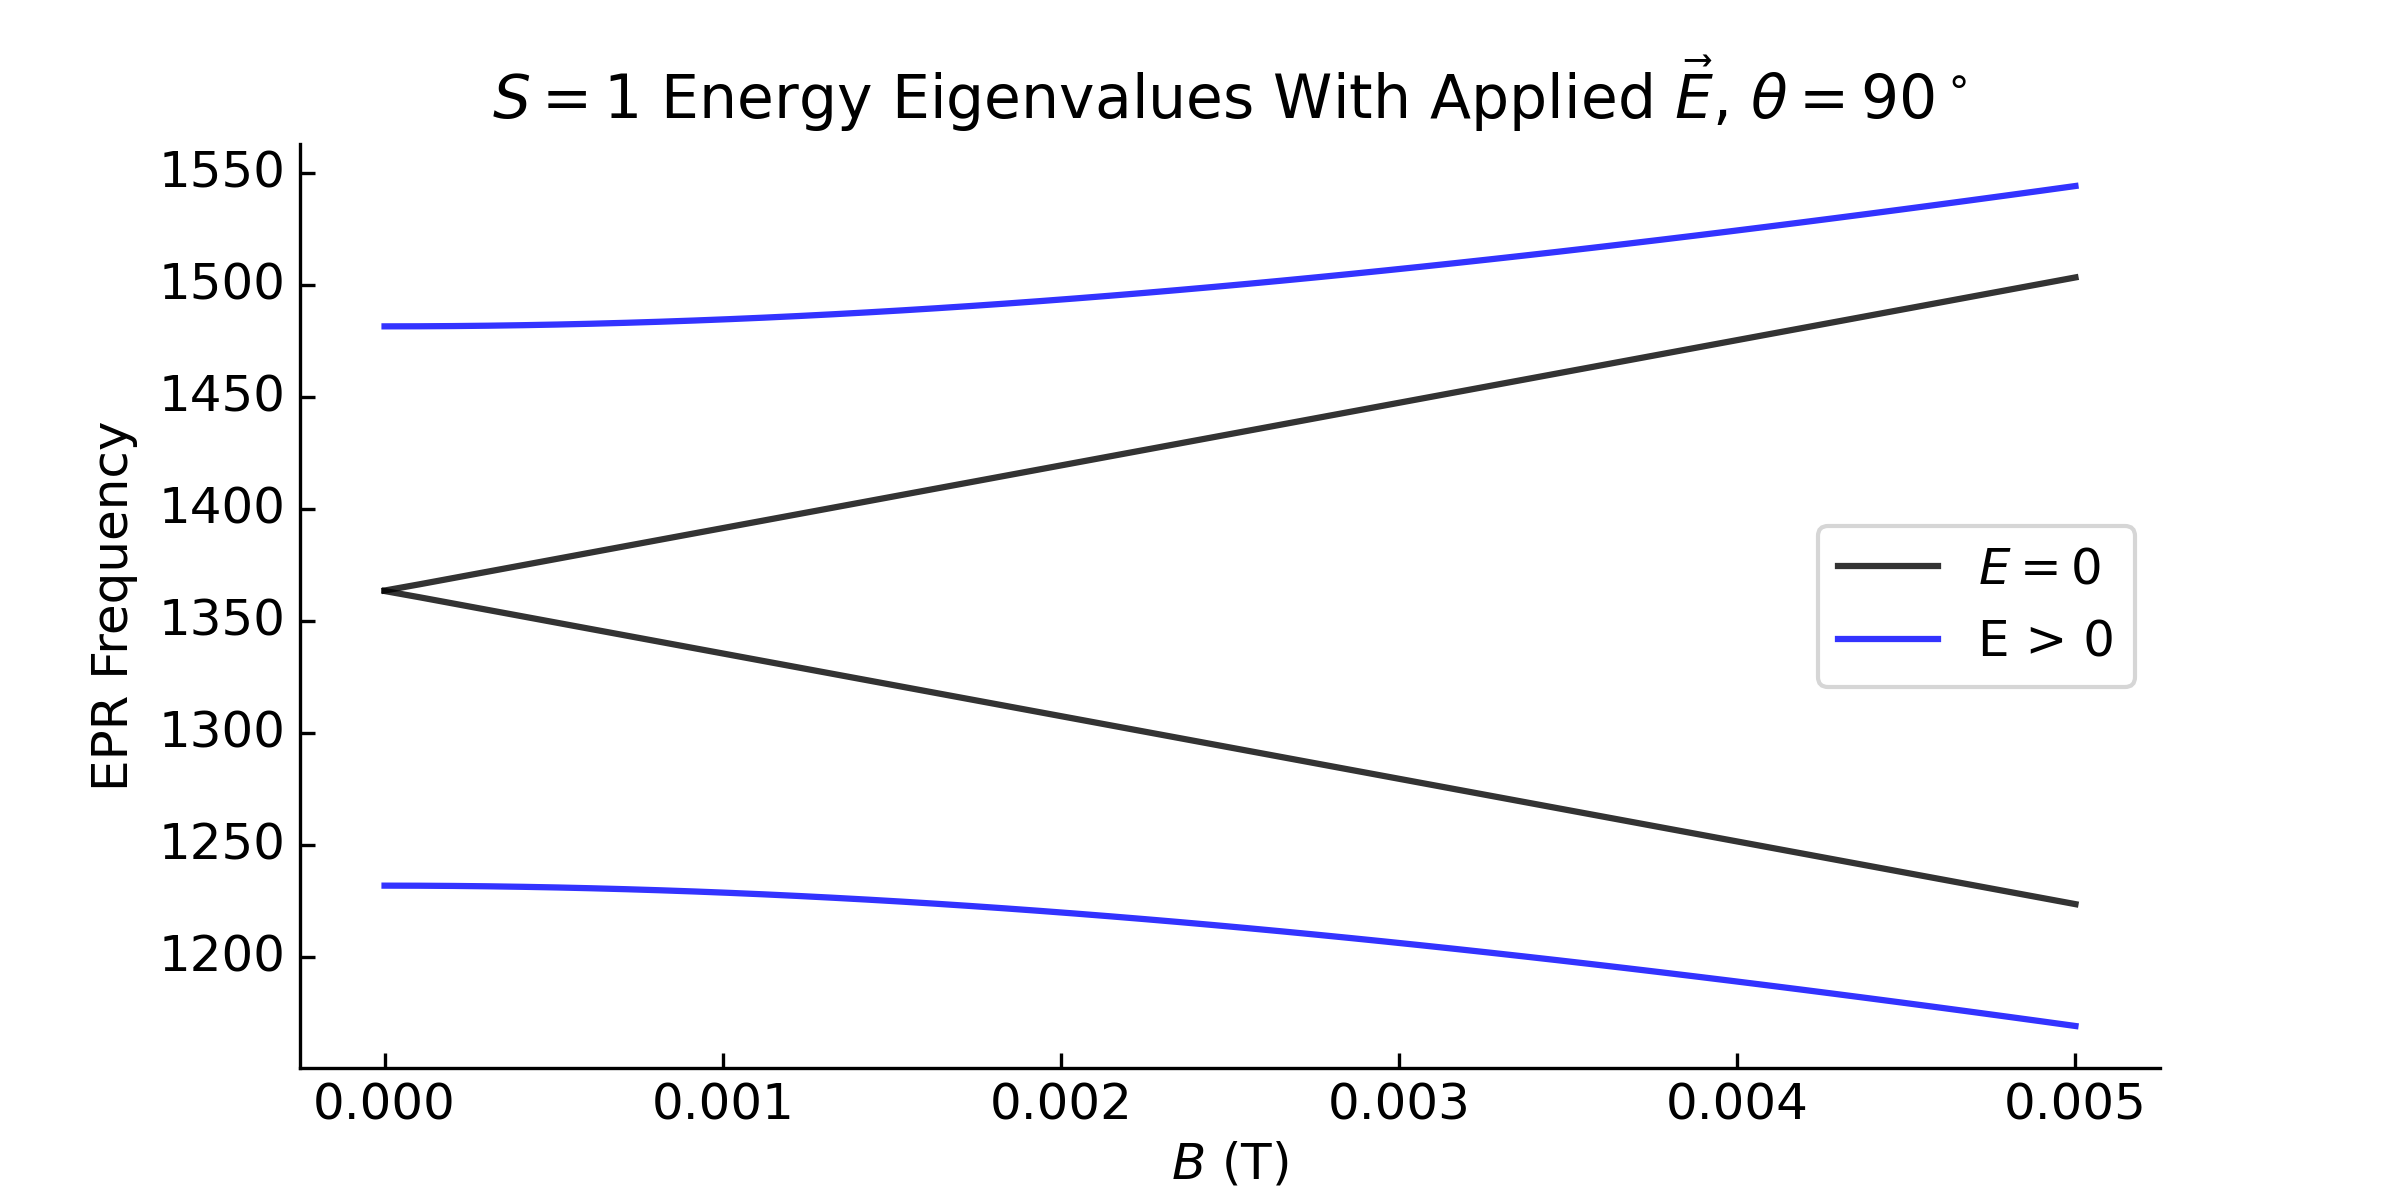
\includegraphics[width=0.95\textwidth]{figures/EFieldPerp.png}
        % \missingfigure{ODMR/Energy plot showing effect of parallel/perp E field}
    \end{center}
    \caption{Eigenvalue plot showing... \td{better caption}}\label{fig:}
\end{figure}



% The spacings
% between ground-state sublevels remain relatively unaf-
% fected by electric fields [34, 35]

% [34] E. van Oort and M. Glasbeek, Chemical Physics Letters
% 168, 529 (1990).
% [35] F. Dolde, H. Fedder, M. Doherty, T. Nöbauer,
% F. Rempp, G. Balasubramanian, T. Wolf, F. Reinhard,
% L. Hollenberg, F. Jelezko, and Others, Nature Physics
% 7, 459 (2011).
